% cd ..\..\Users\NikitaSkybytskyi\Desktop\c3s1\complex-analysis
% cls && pdflatex lec-02.tex && pdflatex lec-02.tex && del lec-02.out, lec-02.log, lec-02.aux && start lec-02.pdf

% \documentclass[a4paper, 12pt]{article}
\usepackage[utf8]{inputenc}
\usepackage[english, ukrainian]{babel}

\usepackage{amsmath, amssymb}
\usepackage{multicol}
\usepackage{graphicx}
\usepackage{float}

\usepackage{amsthm}
\newtheorem{theorem}{Теорема}[subsection]
\newtheorem*{theorem*}{Теорема}
\newtheorem{lemma}{Лема}[subsection]
\newtheorem*{lemma*}{Лема}
\theoremstyle{definition}
\newtheorem*{remark*}{Зауваження}
\newtheorem*{example}{Приклад}

\newcommand{\Max}{\max\limits}
\newcommand{\Sum}{\sum\limits}
\newcommand{\Int}{\int\limits}
\newcommand{\Lim}{\lim\limits}

\newcommand{\RR}{\mathbb{R}}
\newcommand{\ZZ}{\mathbb{Z}}

\newcommand*\diff{\mathop{}\!\mathrm{d}}
\newcommand*\Diff[1]{\mathop{}\!\mathrm{d^#1}}

\DeclareMathOperator{\Real}{Re}
\DeclareMathOperator{\Imag}{Im}

\DeclareMathOperator{\Ln}{Ln}

\DeclareMathOperator{\Arg}{Arg}

\DeclareMathOperator{\Arctan}{Arctan}
\DeclareMathOperator{\Arcsin}{Arcsin}
\DeclareMathOperator{\Arccos}{Arccos}
\DeclareMathOperator{\Arccosh}{Arccosh}
\DeclareMathOperator{\Arctanh}{Arctanh}

\DeclareMathOperator{\arcsinh}{arcsinh}
\DeclareMathOperator{\arccosh}{arccosh}
\DeclareMathOperator{\arctanh}{arctanh}
\DeclareMathOperator{\arccoth}{arccoth}

\newcommand{\varLimsup}{\varlimsup\limits}

\renewcommand{\epsilon}{\varepsilon}
\renewcommand{\phi}{\varphi}

\allowdisplaybreaks
\setlength\parindent{0pt}

\usepackage{xcolor}
\usepackage{hyperref}
\hypersetup{unicode=true,colorlinks=true,linktoc=all,linkcolor=red}

\numberwithin{equation}{section}% reset equation counter for sections
\numberwithin{equation}{subsection}
% Omit `.0` in equation numbers for non-existent subsections.
\renewcommand*{\theequation}{%
  \ifnum\value{subsection}=0 %
    \thesection
  \else
    \thesubsection
  \fi
  .\arabic{equation}%
}


% \begin{document}

\setcounter{section}{1}
\section{Функції комплексної змінної}

У цьому пункті ми введемо найбільш фундаментальні поняття теорії функції комплексної змінної: поняття функції комплексної змінної, її границі, похідної і, нарешті, поняття аналітичної функції. \\

Центральне місце посідає теорема, що встановлює умови диференційовності функції комплексної змінної. Ці умови зазвичай називають \textit{умовами Коші-Рімана}.

\subsection{Геометричні поняття}

\textit{$\epsilon$-околом} точки $a$ називається відкритий круг радіусу $\epsilon$ з центром в $a$, тобто сукупність точок $z$ які задовольняють нерівності $|z - a| < \epsilon$. \\

Множина \textit{відкрита} якщо разом з кожною своєю точкою вона містить якийсь $\epsilon$-окіл цієї точки. Множина називається \textit{зв'язною} якщо для довільних двох точок цієї множини існує ламана яка їх з'єднує і повністю належить множині. \textit{Областю} на комплексній площині називають відкриту і зв'язну множину. \\

\textit{Граничною точкою} області $D$ називається точка яка сама не належить $D$, але у довільному околі якої є точки з $D$. Сукупність граничних точок області називається \textit{границею} цієї області. Область $D$ із приєднаною до неї границею називають \textit{замкнутою областю} і позначають символом $\overline{D}$. \\

Надалі будемо вважати, що границя області складається зі скінченної кількості замкнутих ліній, розрізів, і точок:
\begin{figure}[H]
	\centering
	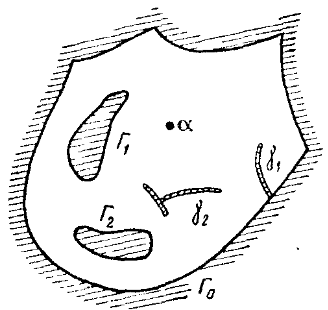
\includegraphics[width=.4\linewidth]{mal-05.png}
	\label{fig:2.1}
\end{figure}

Лінії і розрізи що входять до складу границі будемо вважати \textit{кусково-гладкими}, тобто такими, дотична до яких змінюється неперервно. \\

Область $D$ називається \textit{обмеженою} якщо вона належить якомусь кругу $|z| < R$. Якщо область $D$ обмежена, то кількість зв'язних частин у границі називається \textit{порядком зв'язності} цієї області. Зокрема, якщо границя області $D$ зв'язна, то область $D$ називається \textit{однозв'язною}. \\

\textit{Додатним напрямком обходу} області $D$ вздовж її границі $\Gamma$ називається той, при якому область весь час залишається \textit{ліворуч}. При цьому різні точки границі $\Gamma$ ми відвідаємо різну кількість разів:
\begin{figure}[H]
	\centering
	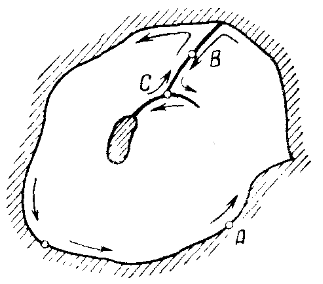
\includegraphics[width=.4\linewidth]{mal-06.png}
	\label{fig:2.2}
\end{figure}
Наприклад, точку $A$ ми відвідаємо один раз, такі точки називаються \textit{простими}, точку $B$ -- двічі, а точку $C$ -- тричі, їх назвемо \textit{кратними} точками, а кількість разів які точка проходиться -- її \textit{кратністю}. \\

Поняття граничної точки \textit{розповсюджується} і на багатозв'язні області.

\subsection{Функції комплексної змінної}

Кажуть, що на множині $M$ точок площини $z$ задана \textit{функція}
\begin{equation}
	\label{eq:2.1.1}
	w = f(z),
\end{equation}
якщо вказано закон, за яким кожній точці $z$ множини $M$ ставиться у відповідність певна точка або сукупність точок $w$. У першому випадку функція $f(z)$ називається \textit{однозначною}, у другому -- \textit{багатозначною}. \\

Множина $M$ називається \textit{множиною визначення} функції $f(z)$, а сукупність $N$ всіх значень $w$ яких $f(z)$ набуває на $M$ -- множиною її значень. Надалі вважатимемо, що $M$ і $N$ -- області. \\

Якщо покласти $z = x + i y$ і $w = u + i v$, то задання функції комплексної змінної $w = f(z)$ буде рівносильним заданню двох функцій від двох дійсних змінних:
\begin{equation}
	\label{eq:2.1.2}
	u = u(x, y), \quad v = v(x, y).
\end{equation}

Будемо позначати значення $z$ на одній комплексній площині, а значення $w$ -- на іншій. Тоді функція комплексно змінної геометрично представляється як \textit{відображення} множини $M$ площини $z$ на множину $N$ площини $w$. \\

Якщо функція $w = f(z)$ однозначна на множині $M$ і довільним двом різним точкам $M$ відповідають різні точки $N$, то відображення називається \textit{взаємно однозначним} або \textit{однолистим}. \\

Нехай задана функція $w = f(z)$ яка відображає множину $M$ на множину $N$. Функція $z = \phi(w)$ яка ставить у відповідність кожній точці $w$ з $N$ сукупність всіх точок $z$ які функцією $w = f(z)$ відображаються у точку $w$ називається \textit{оберненою} до функції $w = f(z)$:
\begin{figure}[H]
	\centering
	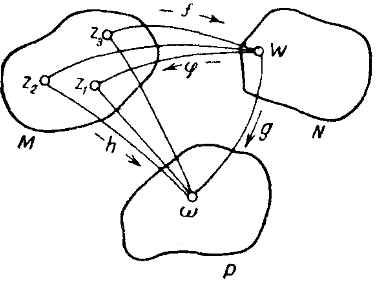
\includegraphics[width=.4\linewidth]{mal-07.png}
	\label{fig:2.3}
\end{figure}

Зрозуміло, що відображення $w = f(z)$ буде взаємно однозначним тоді і лише тоді, коли обидві функції $f$ і $\phi$ однозначні. \\

Нехай функція $w = f(z)$ відображає множину $M$ на $N$, а $\omega = g(w)$ -- множину $N$ на $P$. Функція
\begin{equation}
	\label{eq:2.1.3}
	\omega = h(z) = g(f(z)),
\end{equation}
що відображає $M$ на $P$ називається \textit{складеною функцією}, складеною із $f$ і $g$, а відповідне відображення $h$ -- \textit{суперпозицією} відображень $f$ і $g$. \\

Якщо, зокрема, відображення $w = f(z)$ взаємно однозначне і функція $z = \phi(w)$ -- обернена до $f$, то
\begin{equation}
	\label{eq:2.1.4}
	\phi(f(z)) = z.
\end{equation}

\begin{example}
	\textit{Лінійна функція} визначається у всій площині $z$ співвідношенням

	\begin{equation}
		\label{eq:2.1.5}
		w = a z + b,
	\end{equation}
	де $a \ne 0$ і $b$ -- довільні комплексні сталі. Покладемо $k = |a|$, $\alpha = \Arg a$, тобто $a = k(\cos \alpha + i \sin \alpha)$, і подамо функцію \eqref{eq:2.1.5} як складену функцію, складену з функцій:
	\begin{equation}
		\label{eq:2.1.6}
		z_1 = (\cos \alpha + i \sin \alpha) z; \quad z_2 = k z_1; \quad w = z_2 + b.
	\end{equation}
	Згадуючи геометричний зміст множення, ми бачимо, що перші два відображення зводяться до повороту площини $z$ на кут $\alpha$ і гомотетії площини $z_1$ з центром 0 і коефіцієнтом $k$. Останнє ж відображення є паралельним переносом площини $z_2$ на вектор $b$:
	\begin{figure}[H]
		\centering
		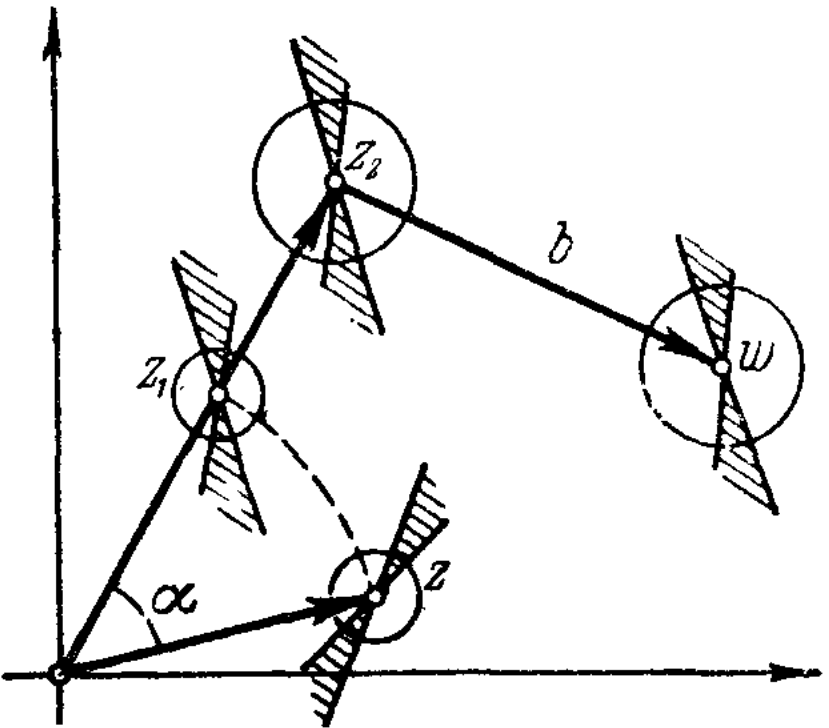
\includegraphics[width=.4\linewidth]{mal-08.png}
		\label{fig:2.3_5}
	\end{figure}
	З того, що лінійне відображення \eqref{eq:2.1.5} є композицією однолистих відображень випливає, що воно і само є однолистим. \\

	Зауважимо також, що воно перетворює прямі у прямі (зберігаючи кути між ними), а кола -- у кола. Інші відображення з такими властивостями будуть детальніше розглянуті пізніше.
\end{example}

\subsection{Диференційовність та аналітичність}

Нехай функція $f(z)$ визначена та однозначна у деякому околі точки $z_0 = x_0 + i y_0$, окрім, можливо, самої точки $z_0$. \\

Будемо казати, що існує \textit{границя функції $f(z)$ при $z \to z_0$} (позначається $\Lim_{z\to z_0} f(z)$) якщо існують границі $\Lim_{\substack{x\to x_0\\y\to y_0}} u(x, y) = u_0$ і $\Lim_{\substack{x\to x_0\\y\to y_0}} v(x, y) = v_0$. \\

Зрозуміло, що
\begin{equation}
	\label{eq:2.2.1}
	\Lim_{z \to z_0} f(z) = u_0 + i v_0 = w_0.
\end{equation}

Оскільки наше визначення зводиться до звичайного визначення границі дійсної функції, то основні властивості граничного переходу \textit{зберігаються}. Зокрема,
\begin{align}
	\label{eq:2.2.2}
	\Lim (f \pm g) &= \Lim f \pm \Lim g, \\
	\label{eq:2.2.3}
	\Lim (f \cdot g) &= \Lim f \cdot \Lim g, \\
	\label{eq:2.2.4}
	\Lim \dfrac{f}{g} &= \dfrac{\Lim f}{\Lim g} \quad (\Lim g \ne 0).
\end{align}

Визначення границі можна також сформулювати за допомогою поняття околу: $\Lim_{z \to z_0} f(z) = w_0$ тоді й тільки тоді, коли для довільного $\epsilon > 0$ знайдеться $\delta > 0$ таке, що для всіх точок із $\delta$-околу точки $z_0$ (окрім, можливо, самої точки $z_0$) відповідні точки $w$ лежать в $\epsilon$-околі точки $w_0$. \\

Іншими словами, $\Lim_{z \to z_0} f(z) = w_0$ якщо з нерівностей
\begin{equation}
	\label{eq:2.2.5}
	0 < |z - z_0| < \delta
\end{equation}
випливає
\begin{equation}
	\label{eq:2.2.6}
	|f(z) - w_0| < \epsilon.
\end{equation}

Функція $f(z)$ прямує до своєї границі \textit{незалежно} від способу прямування точки $z$ до $z_0$. \\

Функція $f(z)$ називається \textit{неперервною в точці $z_0$} якщо вона визначена у деякому околі точки $z_0$ (включаючи саму точку $z_0$) і
\begin{equation}
	\label{eq:2.2.7}
	\Lim_{z \to z_0} f(z) = f(z_0).
\end{equation}

Для неперервності $f(z)$ у точці $z_0$ \textit{необхідно і достатньо} неперервності $u(z, y)$ і $v(x, y)$ в $(x_0, y_0)$. \\

Функція $f(z)$ називається \textit{неперервною в області $D$} якщо вона неперервна в кожній точці цієї області. \\

Визначення неперервності також поширюється на довільну множину $A$, з тією лише поправкою, що тепер $z \to z_0$ по точках $A$. \\

Формально, функція $f(z)$ називається \textit{неперервною на множині $A$} якщо у кожній точці скупчення $z_0 \in A$ існує границя по множині
\begin{equation}
	\label{eq:2.2.8}
	\Lim_{\substack{z \to z_0 \\ z \in A}} f(z) = f(z_0).
\end{equation}

\textit{Компактною} називається обмежена і замкнута множина. \\

Багато властивостей неперервної на інтервалі функції переносяться на неперервну на компакті функцію. А саме, довільна функція $f(z)$ неперервна на компактній множині $\overline{A}$:
\begin{enumerate}
	\item \textit{обмежена на ньому}, тобто існує така стала $M$, що для всіх $z$ із $\overline{A}$ справедливо
	\begin{equation}
		\label{eq:2.2.9}
		|f(z) \le M;
	\end{equation}
	\item \textit{досягає (за модулем) екстремумів}, тобто в $\overline{A}$ існують такі точки $z'$ і $z''$, що для всіх $z$ із $\overline{A}$:
	\begin{equation}
		\label{eq:2.2.10}
		|f(z') \ge |f(z)|, \quad |f(z'')| \le |f(z)|;
	\end{equation}
	\item \textit{рівномірно неперервна}, тобто для довільного $\epsilon > 0$ знайдеться $\delta > 0$ таке, що для довільної пари точок $z_1$ і $z_2$ із $\overline{A}$ яка задовольняє нерівності $|z_1 - z_2| < \delta$, справедлива нерівність
	\begin{equation}
		\label{eq:2.2.11}
		|f(z_1) - f(z_2)| < \epsilon.
	\end{equation}
\end{enumerate}

Також сформулюємо (без доведення) одне твердження, яким неодноразово будемо користуватися надалі:

\begin{theorem}
	Якщо $w = f(z)$ -- неперервна бієкція з області $D$ у множину $\Delta$, то $\Delta$ також область і обернена функція $z = \phi(w)$ неперервна в $\Delta$.
\end{theorem}

Будемо казати, що функція $f(z)$ \textit{диференційовна} в точці $z$ якщо вона визначена в деякому околі точки $z$ і існує границя
\begin{equation}
	\label{eq:2.2.12}
	\Lim_{h \to 0} \dfrac{f(z + h) - f(z)}{h} = f'(z).
\end{equation}
Цю границю будемо називати \textit{похідною} функції $f(z)$ в точці $z$.

\subsubsection{Умови Коші-Рімана}

\begin{theorem}[Умови диференційовності $f(z)$ у термінах дійсних функцій $u(x,y)$ і $v(x,y)$]
	Нехай $f(z) = u(x,y) + i v(x,y)$ визначена в деякому околі точки $z$, причому в цій точці функції $u(x, y)$ і $v(x, y)$ диференційовні, тоді для диференційовності функції комплексної змінної $f(z)$ в точці $z$ необхідно і достатньо, аби в цій точці виконувалися співвідношення
	\begin{align}
		\label{eq:2.2.13}
		\dfrac{\partial u}{\partial x} &= \dfrac{\partial v}{\partial y}, \\
		\label{eq:2.2.14}
		\dfrac{\partial u}{\partial y} &= - \dfrac{\partial v}{\partial x}.
	\end{align}
	Ці умови заведено називати умовами Коші-Рімана.
\end{theorem}

\begin{proof}
	Необхідність. Нехай існує 
	\begin{equation}
		\label{eq:2.2.15}
		f'(z) = \Lim_{h \to 0} \frac{f(z + h) - f(z)}{h}.
	\end{equation}

	Скористаємося зауваження про незалежність границі від способу наближення до точки $z$. Припустимо спершу, що точка $z + h$ наближається до $z$ по прямій, яка паралельна дійсній вісі, тобто $h = s$, $s \to 0$, $s \in \RR$. Тоді отримаємо:
	\begin{multline}
		\label{eq:2.2.16}
		f'(z) = \Lim_{s \to 0} \frac{u(x + s, y) - u(x, y)}{s} + i \cdot \Lim_{s \to 0} \frac{v(x + s, y) - v(x, y)}{s} = \\ = \frac{\partial u}{\partial x} + i \cdot \frac{\partial v}{\partial x}.
	\end{multline}

	Знайдемо тепер ту ж границю у припущенні, що точка $z + h$ наближається до $z$ по прямій, яка паралельна уявній вісі, тобто $h = it$, $t \to 0$, $t \in \RR$. Отримаємо
	\begin{multline}
		\label{eq:2.2.17}
		f'(z) = \Lim_{t \to 0} \frac{u(x, y + t) - u(x, y)}{it} + i \cdot \Lim_{s \to 0} \frac{v(x, y + t) - v(x, y)}{it} = \\ = -i \cdot\frac{\partial u}{\partial y} + \frac{\partial v}{\partial y}.
	\end{multline}

	Прирівнюючи вирази \eqref{eq:2.2.16} і \eqref{eq:2.2.17} для \eqref{eq:2.2.15} отримаємо
	\begin{equation}
		\label{eq:2.2.18}
		\frac{\partial u}{\partial x} + i \cdot \frac{\partial v}{\partial x} = \frac{\partial v}{\partial y} - i \cdot\frac{\partial u}{\partial y}.
	\end{equation}

	Звідси випливаються рівності \eqref{eq:2.2.13} і \eqref{eq:2.2.14} дійсних та уявних частин відповідно.\\

	Достатність. За визначенням диференціалу функції двох дійсних змінних справедливі рівності
	\begin{align}
		\label{eq:2.2.19}
		u(x + s, y + t) - u(x, y) = \frac{\partial u}{\partial x} \cdot s + \frac{\partial u}{\partial y} \cdot t + \alpha \cdot |h|, \\
		\label{eq:2.2.20}
		v(x + s, y + t) - u(x, y) = \frac{\partial v}{\partial x} \cdot s + \frac{\partial v}{\partial y} \cdot t + \beta \cdot |h|,
	\end{align}
	де $\alpha, \beta \to 0$ разом з $h = s + it$. Тоді приріст функції $f(z)$ набуває вигляд:
	\begin{equation}
		\label{eq:2.2.21}
		f(z + h) - f(z) = \frac{\partial u}{\partial x} \cdot s + \frac{\partial u}{\partial y} \cdot t + i \left( \frac{\partial v}{\partial x} \cdot s + \frac{\partial v}{\partial y} \cdot t\right) + \eta \cdot |h|,
	\end{equation}
	де $\eta = \alpha + i \beta$. Використовуючи умови \eqref{eq:2.2.13} та \eqref{eq:2.2.14}, цей приріст можна переписати у вигляді
	\begin{equation}
		\label{eq:2.2.22}
		f(z + h) - f(z) = \left(\frac{\partial u}{\partial x} + i \cdot \frac{\partial v}{\partial x}\right) \cdot (s + it) + \eta \cdot |h| = A h + \eta \cdot |h|,
	\end{equation}
	де $A = \frac{\partial u}{\partial x} + i \cdot \frac{\partial v}{\partial x}$ -- цілком конкретне число, що не залежить від $h$, а $\eta \to 0$ при $h \to 0$. \\

	Розділивши співвідношення \eqref{eq:2.2.22} на $h$ побачимо, що 
	\begin{equation}
		\label{eq:2.2.23}
		\Lim_{h \to 0} \frac{f(z + h) - f(z)}{h}
	\end{equation}
	існує і дорівнює $A$.
\end{proof}

З використанням умов Коші-Рімана похідну функції $f(z)$ можна представити у наступних рівносильних формах:
\begin{equation}
	\label{eq:2.2.24}
	f'(z) = \dfrac{\partial u}{\partial x} + i \cdot \dfrac{\partial v}{\partial x} = \dfrac{\partial v}{\partial y} - i \cdot \dfrac{\partial u}{\partial y} = \dfrac{\partial u}{\partial x} - i \cdot \dfrac{\partial u}{\partial y} = \dfrac{\partial v}{\partial y} + i \cdot \dfrac{\partial v}{\partial x}.
\end{equation}

Оскільки звичайні властивості алгебраїчних дій і граничного переходу зберігаються, то зберігаються і звичайні правила диференціювання, тобто:
\begin{align}
	\label{eq:2.2.25}
	(f \pm g)' &= f' \pm g', \\
	\label{eq:2.2.26}
	(f \cdot g)' &= f' \cdot g + f \cdot g', \\
	\label{eq:2.2.27}
	\left(\dfrac fg\right)' &= \dfrac{f' \cdot g - f \cdot g'}{g^2}, \\
	\label{eq:2.2.28}
	f(g(z))' &= f'(g(z)) \cdot g'(z), \\
	\label{eq:2.2.29}
	f'(z) \cdot \phi'(w) &= 1.
\end{align}

Функція $f(z)$ диференційовна у кожній точці області $D$ називається \textit{аналітичною} (\textit{регулярною} або \textit{голоморфною}) у цій області. \\

Зауважимо також, що умови Коші-Рімана виконуються якщо замість $x$ і $y$ взяти довільні два перпендикулярні ($n = is$) напрямки $n$ і $s$, тобто
\begin{align}
	\label{eq:2.2.30}
	\dfrac{\partial u}{\partial s} &= \dfrac{\partial v}{\partial n}, \\
	\label{eq:2.2.31}
	\dfrac{\partial u}{\partial n} &= - \dfrac{\partial v}{\partial s}.
\end{align}

Умови Коші-Рімана також мають запис у полярних координатах:
\begin{align}
	\label{eq:2.2.32}
	\dfrac{\partial u}{\partial \phi} &= - r \cdot \dfrac{\partial v}{\partial r}, \\
	\label{eq:2.2.33}
	r \cdot \dfrac{\partial u}{\partial r} &= \dfrac{\partial v}{\partial \phi}.
\end{align}

% \flushright{\copyright \, М. А. Лаврентьев, Б. В. Шабат, 1972 \\ Українською переклав Н. М. Скибицький, 2018}

% \end{document}